\variant
\\
\begin{minipage}[t]{3in}
A 300 mm beam with uniform cross-sectional area 30 mm$^2$ and Young's modulus 30 GPa is constrained to not displace at the ends $A$ and $B$; it experiences a 30 kN load to the left, 100 mm from $B$. What is the reaction force at $B$?
\end{minipage}
\quad
\begin{minipage}[t]{3in}
\vspace{-24pt}
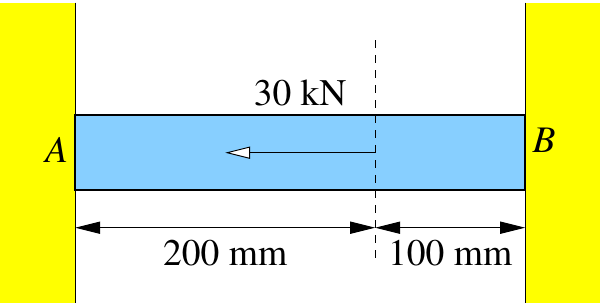
\includegraphics[width=\textwidth]{ch09-bar-load-30}
\end{minipage}
\vspace{-12pt}
\begin{answers}
\answer 10 kN
\correctanswer 20 kN
\answer 30 kN
\answer 60 kN
\answer 120 kN
\end{answers}
\begin{solution}
Take the reaction force at $F_A$ to the right (compressive), and $F_B$ to the right (tensile); then equilibrium requires
\[
F_A + F_B = 30\text{ kN}.
\]
The displacement constraint requires that the displacement from the compressive and tensile portions cancel out, or
\[
\begin{split}
\delta_{A} + \delta_B &= 0\\
-\frac{F_A(200\text{ mm})}{AE} + \frac{F_B(100\text{ mm})}{AE} &= 0\\
F_B &= 2F_A.
\end{split}
\]
Then, $\frac12 F_B + F_B = 30\text{ kN}$, or $F_B = 20\text{ kN}$.
\end{solution}

\variant
\\
\begin{minipage}[t]{3in}
A 300 mm beam with uniform cross-sectional area 30 mm$^2$ and Young's modulus 60 GPa is constrained to not displace at the ends $A$ and $B$; it experiences a 60 kN load to the left, 100 mm from $B$. What is the reaction force at $B$?
\end{minipage}
\quad
\begin{minipage}[t]{3in}
\vspace{-24pt}
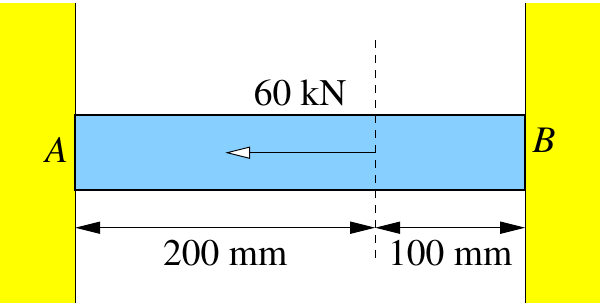
\includegraphics[width=\textwidth]{ch09-bar-load-60}
\end{minipage}
\vspace{-12pt}
\begin{answers}
\answer 20 kN
\correctanswer 40 kN
\answer 60 kN
\answer 120 kN
\answer 240 kN
\end{answers}
\begin{solution}
Take the reaction force at $F_A$ to the right (compressive), and $F_B$ to the right (tensile); then equilibrium requires
\[
F_A + F_B = 60\text{ kN}.
\]
The displacement constraint requires that the displacement from the compressive and tensile portions cancel out, or
\[
\begin{split}
\delta_{A} + \delta_B &= 0\\
-\frac{F_A(200\text{ mm})}{AE} + \frac{F_B(100\text{ mm})}{AE} &= 0\\
F_B &= 2F_A.
\end{split}
\]
Then, $\frac12 F_B + F_B = 60\text{ kN}$, or $F_B = 40\text{ kN}$.
\end{solution}

\variant
\\
\begin{minipage}[t]{3in}
A 300 mm beam with uniform cross-sectional area 30 mm$^2$ and Young's modulus 90 GPa is constrained to not displace at the ends $A$ and $B$; it experiences a 90 kN load to the left, 100 mm from $B$. What is the reaction force at $B$?
\end{minipage}
\quad
\begin{minipage}[t]{3in}
\vspace{-24pt}
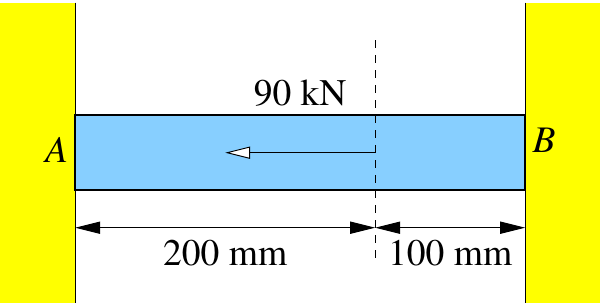
\includegraphics[width=\textwidth]{ch09-bar-load-90}
\end{minipage}
\vspace{-12pt}
\begin{answers}
\answer 30 kN
\correctanswer 60 kN
\answer 90 kN
\answer 180 kN
\answer 360 kN
\end{answers}
\begin{solution}
Take the reaction force at $F_A$ to the right (compressive), and $F_B$ to the right (tensile); then equilibrium requires
\[
F_A + F_B = 90\text{ kN}.
\]
The displacement constraint requires that the displacement from the compressive and tensile portions cancel out, or
\[
\begin{split}
\delta_{A} + \delta_B &= 0\\
-\frac{F_A(200\text{ mm})}{AE} + \frac{F_B(100\text{ mm})}{AE} &= 0\\
F_B &= 2F_A.
\end{split}
\]
Then, $\frac12 F_B + F_B = 90\text{ kN}$, or $F_B = 60\text{ kN}$.
\end{solution}

